\chapter{Laboratorio de pruebas}
\label{chapter6}

% **************************** Define Graphics Path **************************
\ifpdf
    \graphicspath{{Chapter6/Figs/Raster/}{Chapter6/Figs/PDF/}{Chapter6/Figs/}}
\else
    \graphicspath{{Chapter6/Figs/Vector/}{Chapter6/Figs/}}
\fi

Para validar funcionalmente el prototipo es preciso la construcción de un laboratorio de experimentación sobre el cual ejecutar un conjunto de pruebas e implementar algunos casos de uso representativos. Dentro de las pruebas funcionales se busca verificar aspectos importantes de la implementaci\'on como la clasificación de tr\'afico, el algoritmo de ruteo dinámico y el algoritmo de distribución de etiquetas.

Por otro lado con la implementaci\'on de algunos casos de uso representativos se busca validar la utilización del enfoque OpenFlow/SDN en la construcci\'on a futuro de la RAU2.\\

El siguiente capitulo esta destinado a la presentación del laboratorio de pruebas construido y a la descripción de las diferentes pruebas realizadas.

% **************************** Construccion del TestBed ************************** 
\section{Definición del Laboratorio}

Como se menciona anteriormente uno de los objetivos de este laboratorio de experimentaci\'on es verificar el correcto funcionamiento de la implementaci\'on realizada, en particular en los aspectos críticos de la misma como la capacidad para clasificar trafico y los diferentes algoritmos de ruteo, distribución de etiquetas, actualización topologica, etc. 

Para esto es necesario construir un prototipo con suficientes nodos y enlaces como para poder definir varios servicios de redes privadas. Tambi\'en interesa la existencia de caminos alternativos entre un par de nodos origen y destino para poder comprobar el funcionamiento del algoritmo de ruteo y evaluar el comportamiento del prototipo cuando la topolog\'ia cambia, desconectando enlaces, apagando nodos, etc.\\

Teniendo en cuanta los requerimientos mencionados se construye un laboratorio de pruebas con la siguiente topolog\'ia (ver figura \ref{fig:LaboratorioDePruebasTopo}).
  
\begin{figure}[ht!] 
\centering    
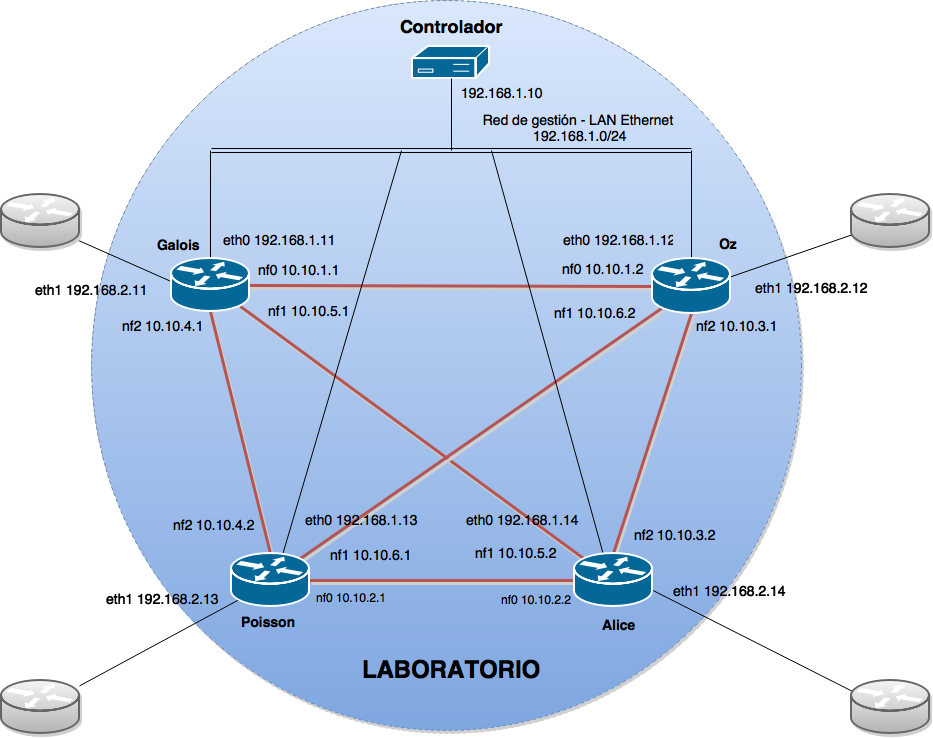
\includegraphics[width=0.85\textwidth]{Topologia}
\caption[Laboratorio de pruebas - Topolog\'ia]{Laboratorio de pruebas - Topolog\'ia}
\label{fig:LaboratorioDePruebasTopo}
\end{figure}

El laboratorio se compone de cuatro nodos implementados en base al dispositivo RAU-Switch conectados entre si con enlaces de fibra \'optica multimodo. Cada nodo esta conectado a los otros tres nodos de la topolog\'ia implementando de esta forma una topolog\'ia full mesh de cuatro nodos.

A su vez cada nodo esta conectado al controlador SDN del prototipo mediante una interfaz de red de 10Mb (interfaces \textbf{eth0}).\\

Por la forma que tiene la topolog\'ia, los cuatro nodos nombrados \textit{Galois}, \textit{Poisson}, \textit{Oz} y \textit{Alice} son nodos de borde. Esto quiere decir que RAUFlow los considera como nodos habilitados para ser nodo de ingreso \'o nodo de egreso en la definici\'on de servicios de redes privadas.

Por otro lado cada nodo cuenta con una interfaz de red de 100Mb (interfaz \textbf{eth1}) utilizada como interfaz externa para la conexi\'on con otras subredes. Estas interfaces son utilizadas por RAUFlow para la definici\'on de servicios de VPN como los puntos de entrada y salida de tr\'afico. Por tanto cada una de estas interfaces se encuentra directamente conectada a la subred de una VPN en particular.\\  

Como se menciona anteriormente en lacp\'itulo 5, la representaci\'on utilizada para modelar una topolog\'ia de red es la de un multigrafo dirigido ponderado. En la figura \ref{fig:LaboratorioDePruebasCostos} se muestra esta representaci\'on para la topolog\'ia del prototipo. Como puede apreciarse en la im\'agen cada enlace tiene su respectivo costo asociado.

Por simplicidad en el diagrama se han obviado los enlaces existentes entre el Controlador y cada uno de los nodos. Como se menciona en el cap\'itulo 4 la instancia de Quagga ejecutada en el controlador tiene como \'unico objetivo contar con un acceso local a la LSDB. Por ello conceptualmente el costo asociado a cada uno de estos enlaces es infinito, lo cual en pr\'actica se realiza asignando el valor 65535.  

\begin{figure}[ht!] 
\centering    
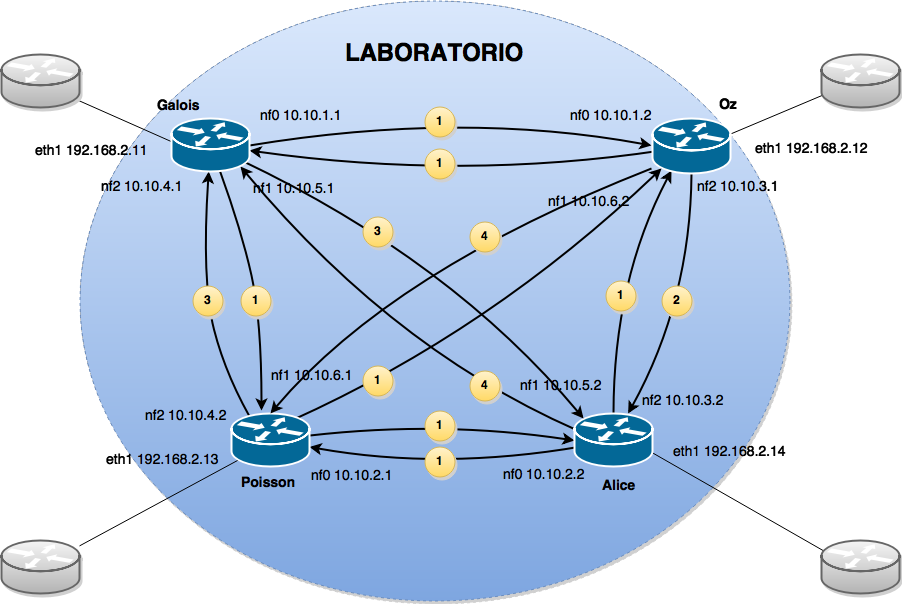
\includegraphics[width=0.85\textwidth]{TopologiaCostos}
\caption[Laboratorio de pruebas - Costos de la topolog\'ia]{Laboratorio de pruebas - Costos de la topolog\'ia}
\label{fig:LaboratorioDePruebasCostos}
\end{figure}

Sobre este laboratorio se implementan dos casos de uso representativos: (a) VPN de capa 3 y (b) VPN de capa 2. Sobre cada uno de estos casos de uso a su vez se ejecutan una serie de pruebas orientadas a verificar el correcto funcionamiento de las componentes m\'as importantes en la implementaci\'on de RAUFlow y RAU-Switch.

A continuaci\'on se describen los resultados obtenidos en la implementaci\'on de estos casos de uso y la eecuci\'on de estas pruebas, comenzando por el caso de uso VPN de capa 3.

\section{VPN de capa 3}

Las redes privadas virtuales de capa 3 son un tipo de servicio comunmente brindado por un operador de red y es en particular uno de los servicios que se quiere implementar en la RAU2. En particular con este tipo de red privada se puede implementar clasificaci\'on de tr\'afico en base a tipo de aplicaci\'on y numeraci\'on de capa 3.\\

En este trabajo se implementan dos escenarios diferentes para este tipo de red privada: (a) red privada multipunto con una \'unica organizaci\'on y tres sucursales f\'isicamente separadas, (b) red privada punto a punto con dos organizaciones, cada una de ellas con dos sucursales f\'isicamente separadas.

\subsection{Escenario 1 - Red Privada Multipunto}

Este escenario representa una red privada multipunto de capa 3. Esta compuesto por una \'unica organizaci\'on o red privada dividida en 3 sucursales o subredes.

\begin{figure}[ht!] 
\centering    
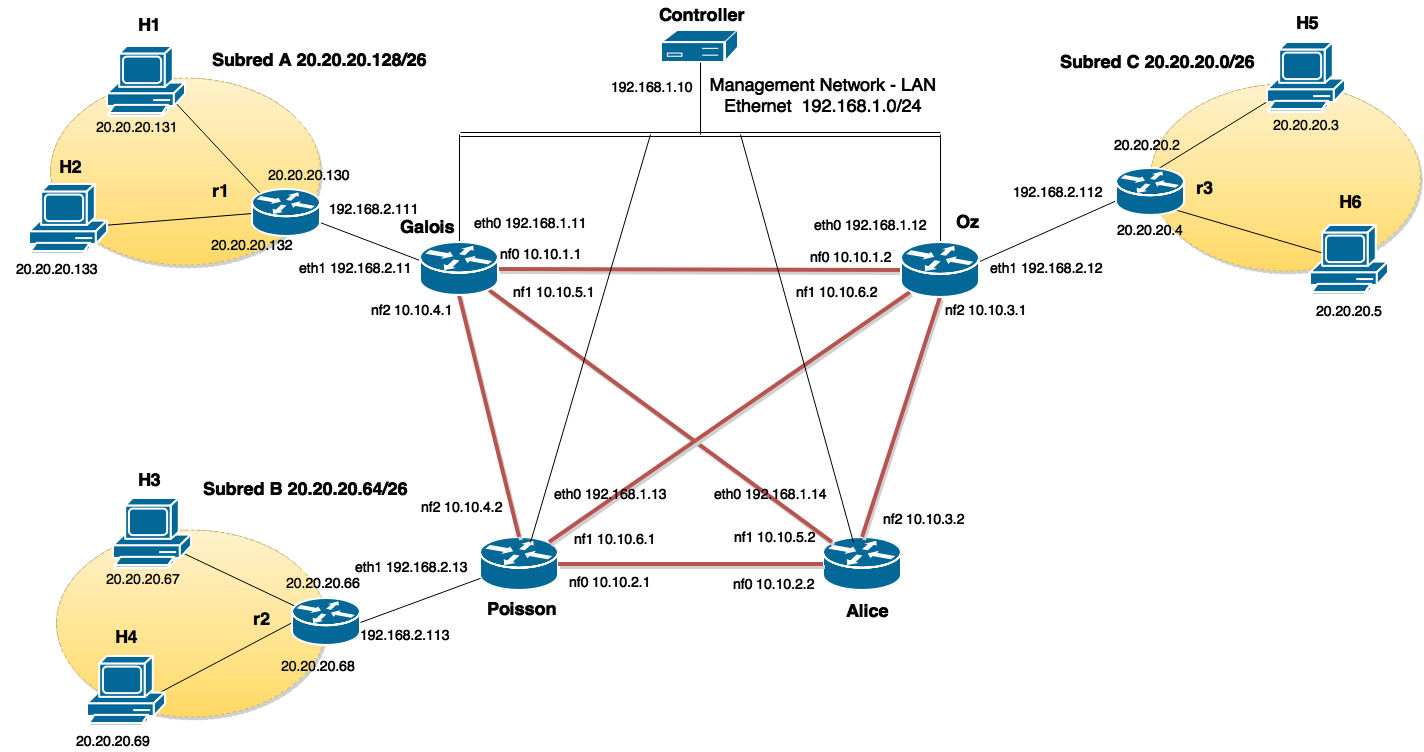
\includegraphics[width=1.0\textwidth]{CU1P1}
\caption[VPN de capa 3 - Escenario 1]{VPN de capa 3 - Escenario 1}
\label{fig:CUP1}
\end{figure}

Sobre este escenario se ejecutan una serie de pruebas orientadas a verificar los siguientes aspectos relacionados al prototipo:

\begin{enumerate}
\item Algoritmo de ruteo
\item Algoritmo de distribución de etiquetas
\item Clasificaci\'on de tr\'afico
\item Actualizaci\'on de rutas cuando cambia la topolog\'ia
\item Capacidad para crear VPN multipunto
\end{enumerate}

Para construir la red privada multipunto uniendo las tres subredes mencionadas y adem\'as verificar los puntos anteriores, se instancian los siguientes servicios(ver tabla \ref{table:TablaFlujos}). Por cada par de subredes se crean dos servicios (un servicio para cada sentido del tr\'afico).\\

\begin{table}[h]
\begin{tabular}{| l | l | l | p{4cm} | p{4cm} |}
\hline
Nombre & Ingreso & Egreso & Clasificación & Descripción \\ \hline

\crule[Aquamarine]{0.3cm}{0.3cm} S1 & Galois - eth1 & Oz - eth1 & ip\_src=20.20.20.128/26 ip\_dst=20.20.20.0/26 & Tr\'afico de Subred A a Subred C \\ \hline

\crule[Red]{0.3cm}{0.3cm} S2 & Oz - eth1 & Galois - eth1 & ip\_src=20.20.20.0/26 ip\_dst=20.20.20.128/26 & Tr\'afico de Subred C a Subred A \\ \hline

\crule[ForestGreen]{0.3cm}{0.3cm} S3 & Galois - eth1 & Poisson - eth1 & ip\_src=20.20.20.128/26 ip\_dst=20.20.20.64/26 & Tr\'afico de Subred A a Subred B \\ \hline

\crule[LimeGreen]{0.3cm}{0.3cm} S4 & Poisson - eth1 & Galois - eth1 & ip\_src=20.20.20.64/26 ip\_dst=20.20.20.128/26 & Tr\'afico de Subred B a Subred A \\ \hline

\crule[RoyalPurple]{0.3cm}{0.3cm} S5 & Poisson - eth1 & Oz - eth1 & ip\_src=20.20.20.64/26 ip\_dst=20.20.20.0/26 & Tr\'afico de Subred B a Subred C \\ \hline

\crule[YellowOrange]{0.3cm}{0.3cm} S6 & Oz - eth1 & Poisson - eth1 & ip\_src=20.20.20.0/26 ip\_dst=20.20.20.64/26 & Tr\'afico de Subred C a Subred B \\ \hline
\end{tabular}
\vspace{0.3cm}
\caption[CU1 - Escenario 1, servicios creados]{CU1 - Escenario 1, servicios creados}
\label{table:TablaFlujos}
\end{table}

Para cada uno de estos servicios adem\'as se indica el etherype 0x0800 correspondiente al tipo de tr\'afico IPv4.\\

\subsubsection{Verificaci\'on de Algoritmo de ruteo}
Para verificar el correcto funcionamiento del algoritmo de ruteo, se comparan los caminos calculados para cada servicio con los respectivos mejores caminos te\'oricos. 

Para cada camino se verifican dos cosas: (1) que el camino calculado se corresponde con el camino te\'orico y (2) que el camino es correctamente instalado como reglas de reenvío (en base a conmutaci\'on de etiquetas) en la tabla de flujos OpenFlow de cada nodo del camino.\\

Los caminos te\'oricos son calculados manualmente observando los costos de la topolog\'ia (figura \ref{fig:LaboratorioDePruebasCostos}). Los resultados de este procedimiento se muestran en la figura
 \ref{fig:CUP1Caminos}.\\

\begin{figure}[ht!] 
\centering    
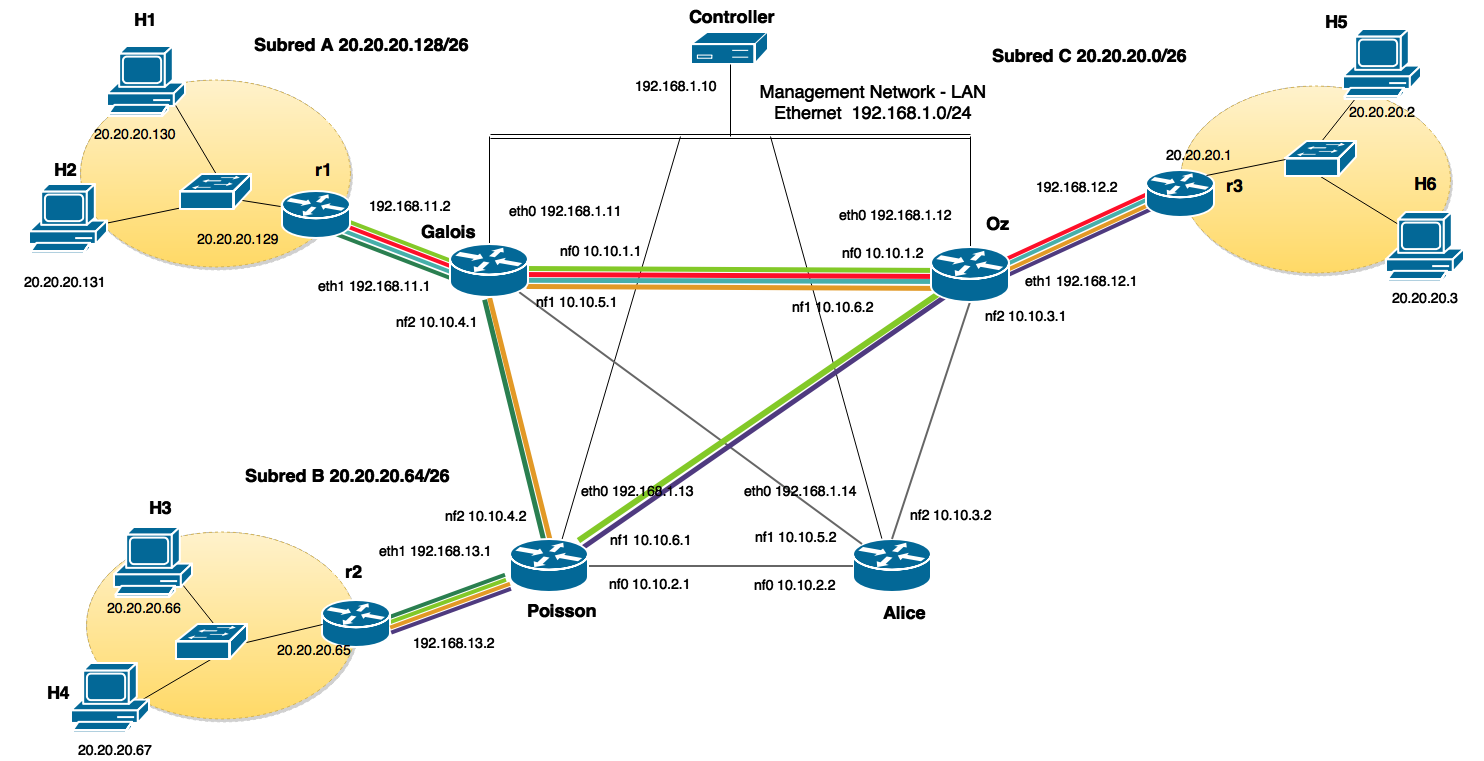
\includegraphics[width=1.0\textwidth]{CU1P1Caminos}
\caption[Escenario 1 - Caminos para servicios]{Escenario 1 - Caminos para servicios}
\label{fig:CUP1Caminos}
\end{figure}

Para comprobar que los caminos calculados por el algoritmo sean los correctos se analizan las tablas de flujos de Open vSwitch en cada nodo de la red del laboratorio. A partir del contenido de estas tablas fácilmente puede reconocerse el camino calculado.\\

En las figuras ~\ref{fig:CU1P1DumpFlows1}~-~\ref{fig:CU1P1DumpFlows4} se muestran las tablas de flujos asociadas a cada nodo. Para conseguir esta informaci\'on se utiliza el comando dump-flows de la herrmaienta Open vSwitch. No obstante puede obtenerse tambi\'en esta informaci\'on de la propia interfaz gr\'afica de RAUFlow.\\

Tomando como ejemplo el caso del servicio S5, acorde al camino te\'orico todo tr\'afico con origen en la Subred B y destino Subred C es encaminado por el enlace que conecta directamente a ambos nodos por las respectivas interfaces \textit{nf1}. 

Asumiendose de aqu\'i en m\'as la notaci\'on $(n, i)$ para referirse a un enlace, donde \textit{n} indica nodo origen e \textit{i} interfaz de reenvío en \textit{n} para el próximo salto, $<(n_1, i_1), \dots, (n_k, i_k)>$ para representar un camino, entonces el camino te\'orico para S5 es el siguiente:

 
$$<(Poisson, nf_1)>$$

\begin{figure}[ht!] 
\centering    
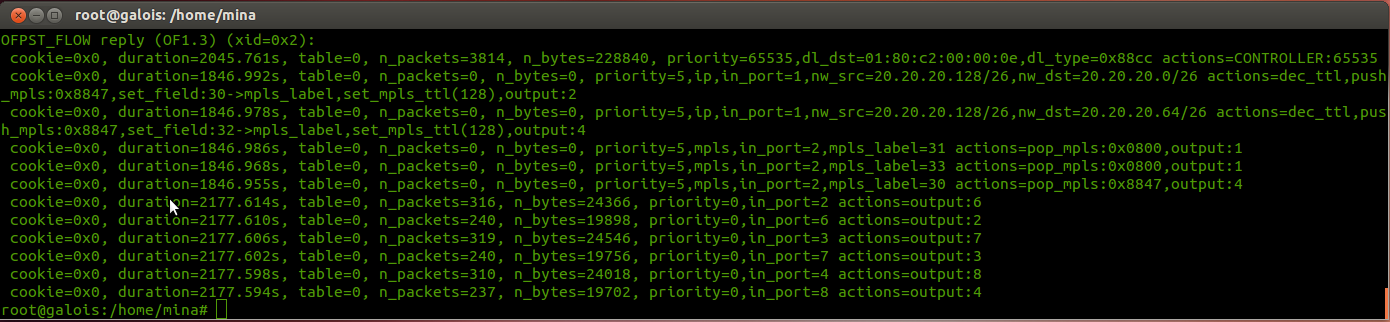
\includegraphics[width=1.0\textwidth]{E1P1Gal}
\caption[Tabla de flujos ovs - Galois]{Tabla de flujos ovs - Galois}
\label{fig:CU1P1DumpFlows1}
\end{figure}

\begin{figure}[ht!] 
\centering    
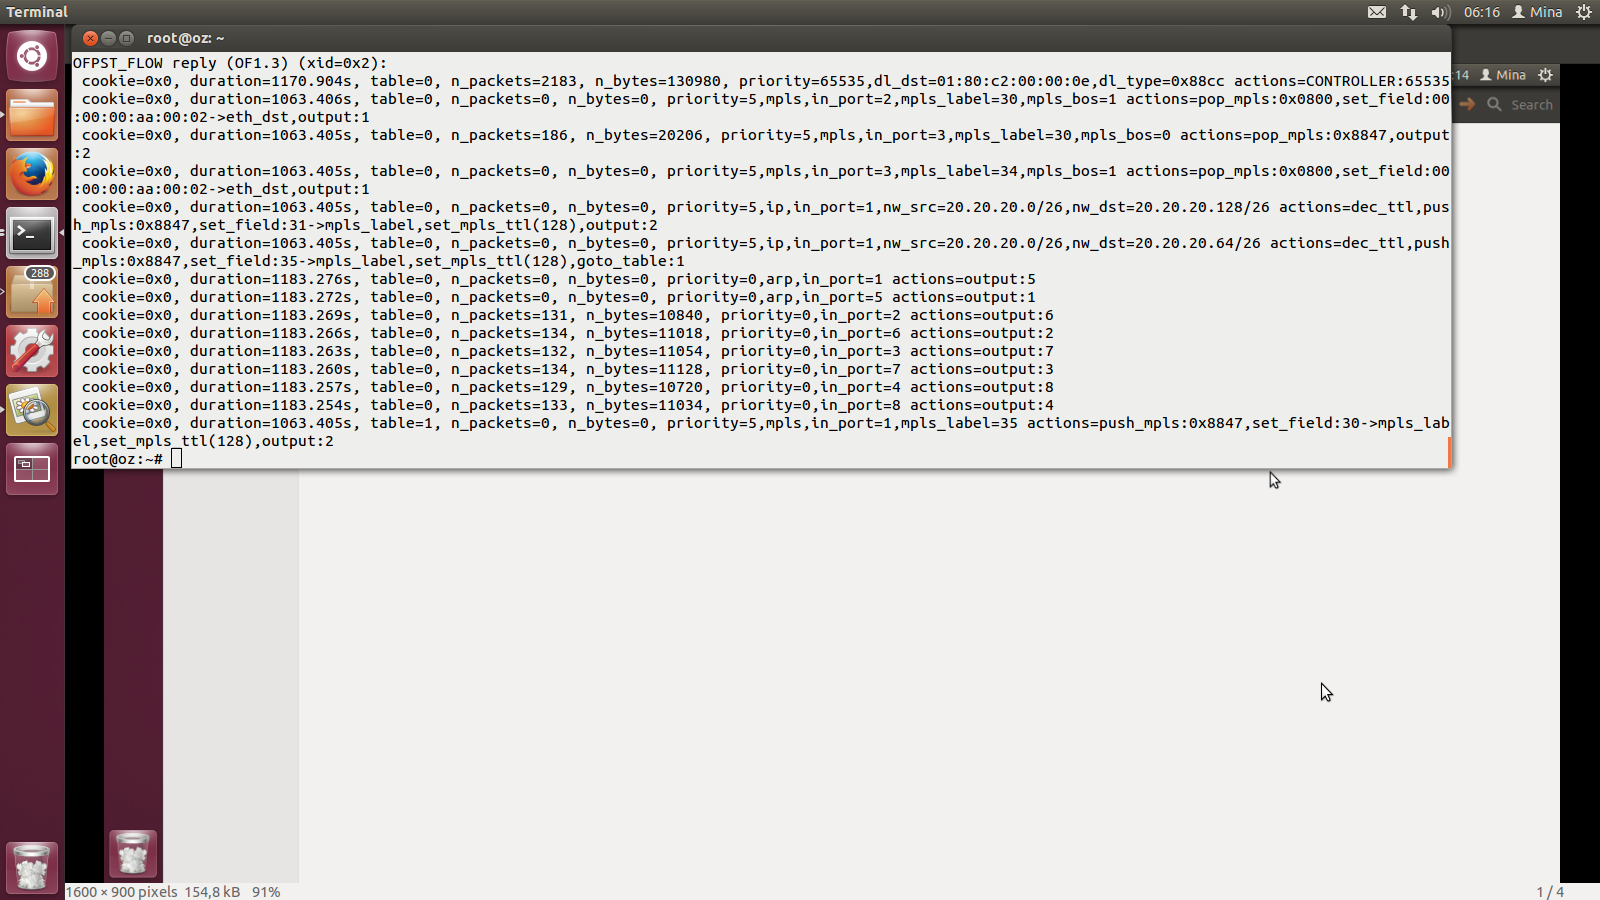
\includegraphics[width=1.0\textwidth]{E1P1Oz}
\caption[Tabla de flujos ovs - Oz]{Tabla de flujos ovs - Oz}
\label{fig:CU1P1DumpFlows2}
\end{figure}

\begin{figure}[ht!] 
\centering    
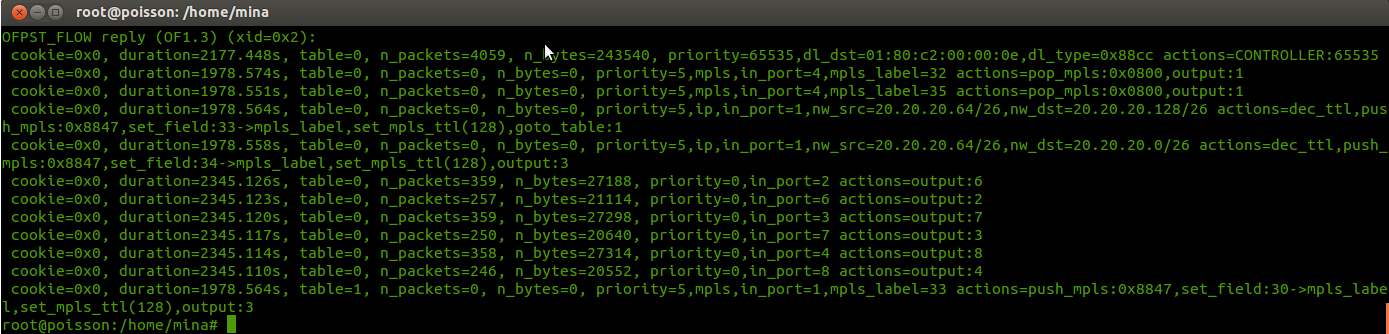
\includegraphics[width=1.0\textwidth]{E1P1Poi}
\caption[Tabla de flujos ovs - Poisson]{Tabla de flujos ovs - Poisson}
\label{fig:CU1P1DumpFlows3}
\end{figure}

\begin{figure}[ht!] 
\centering    
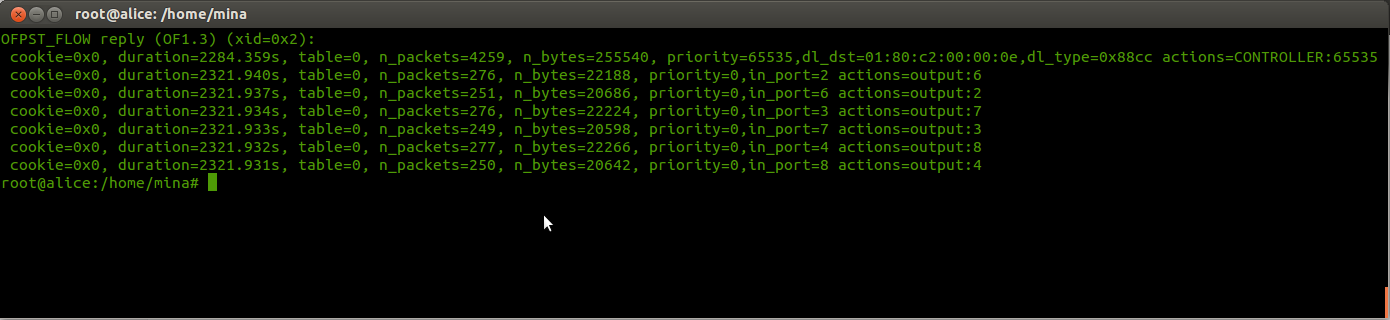
\includegraphics[width=1.0\textwidth]{E1P1Al}
\caption[Tabla de flujos ovs - Alice]{Tabla de flujos ovs - Alice}
\label{fig:CU1P1DumpFlows4}
\end{figure}

[Aca describo los flujos en la tablas de Poisson que hacen que el trafico sea encapsulado y enviado por nf1, y luego los lujos en Oz que desencapsulan el trafico y lo reenvian por eth1 a la subred C implementando de esta forma el camino <Poisson, nf1>]\\

Por otro lado si se toma como ejemplo el servicio S6, seg\'un los costos de la topolog\'ia el camino deber\'ia de ser:

$$<(Oz, nf_0), (Poisson, nf_2)>$$ 

Analizando las tablas de flujos de los nodos \textit{Oz}, \textit{Galois} y \textit{Poisson}, puede comprobarse fácilmente la correspondencia entre el camino calculado y el camino te\'orico.
Por un lado, acorde a la defrinci\'on de servicios, Galois debería reenviar todo tr\'afico de tipo \textbf{ip} que ingresa por la interfaz eth1(la cual se corresponde con el n\'umero de puerto openflow 1), con origen en la subred 20.20.20.64/26 y destino 20.20.20.0/64 por la interfaz nf1(la cual se corresponde con el n\'umero de puerto openflow 3).

Observando la tabla de flujos del nodo Poisson, puede apreciarse el siguiente flujo, con el cual se implementa dicho comportamiento:

\begin{center}
\textit{cookie=0.0, duration=1978.558s, table=0, n\_packets=0, n\_bytes=0, priority=5, \\
ip,in\_port=1, nw\_src=20.20.20.64/26,nw\_dst=20.20.20.0/26 \\
actions=dec\_ttl,push\_mpls:0x8847,set\_field:34->mpls\_label,set\_mpls\_ttl(128),output:3 }
\end{center}

Notese adem\'as la acci\'on \textbf{dec\_ttl} en el flujo. Esta acci\'on es utilizada en cada nodo de borde en la definici\'on de un servicio para decrementar el ttl de un paquete ip cada vez que ingresa a la red del prototipo (en este caso a la red del laboratorio). Observese tambi\'en el valor de la etiqueta mpls(34) colocado en el paquete para identificar el servicio(etiqueta interna).

Por otro lado, una vez que los paquetes asociados al servicio S5 llegan a nodo Oz ingresando por la interfaz nf1(puerto openflow 3), debe ser retirada la etiqueta mpls interna y reenviarse a traves de la interfaz eth1(puerto openflow 1).

Este comportamiento es implementado en la tabla de flujos de Oz por el siguiente flujo:

\begin{center}
\textit{cookie=0.0, duration=1978.558s, table=0, n\_packets=0, n\_bytes=0, priority=5, \\
mpls,in\_port=3,mpls\_label=34 \\
actions=pop\_mpls:0x0800,output:1 }
\end{center}

Como indica el lujo anterior, a todo paquete mpls que ingresa por el puerto openflow 3 y con valor de etiqueta mpls 34, se le retira el cabezal mpls y se lo reenvia por la interfaz eth1(puerto openflow 1). 

\subsubsection{Verificaci\'on de Algoritmo de distribución de etiquetas}

[De repente comentar en funcion al escenario anterior porque anda bien]

\subsubsection{Clasificaci\'on de tr\'afico}
Se implementa clasificaci\'on de tr\'afico en el nodo de borde identificado como ingreso para el tr\'afico de un servicio en concreto. En particular para el escenario con el que se viene trabajando, se implementa clasificaci\'on de tr\'afico en los nodos de ingreso basándose en la numeraci\'on IP origen y destino de un paquete. De esta forma por ejemplo el nodo Galois determina que camino debe tomar un paquete con origen en la Subred A y destino la Subred B. 

Sin embargo RAUFlow admite realizar clasificaci\'on de tr\'afico por un conjunto bastante m\'as amplio de atributos. A continuaci\'on se definen una nueva lista de servicios orientados a demostrar la correcta implementaci\'on de esta funcionalidad.

Cabe destacar que para esta prueba los servicios anteriormente creados son eliminados.

\begin{table}[h]
\begin{tabular}{| l | l | l | p{4cm} | p{4cm} |}
\hline
Nombre & Ingreso & Egreso & Clasificación & Descripción \\ \hline

\crule[Aquamarine]{0.3cm}{0.3cm} S1 & Galois - eth1 & Oz - eth1 & ip\_src=20.20.20.128/26 ip\_dst=20.20.20.0/26 & Tr\'afico de Subred A a Subred C \\ \hline

\crule[Red]{0.3cm}{0.3cm} S2 & Oz - eth1 & Galois - eth1 & ip\_src=20.20.20.0/26 ip\_dst=20.20.20.128/26 & Tr\'afico de Subred C a Subred A \\ \hline

\crule[ForestGreen]{0.3cm}{0.3cm} S3 & Galois - eth1 & Poisson - eth1 & ip\_src=20.20.20.128/26 ip\_dst=20.20.20.64/26 & Tr\'afico de Subred A a Subred B \\ \hline

\crule[LimeGreen]{0.3cm}{0.3cm} S4 & Poisson - eth1 & Galois - eth1 & ip\_src=20.20.20.64/26 ip\_dst=20.20.20.128/26 & Tr\'afico de Subred B a Subred A \\ \hline

\crule[RoyalPurple]{0.3cm}{0.3cm} S5 & Poisson - eth1 & Oz - eth1 & ip\_src=20.20.20.64/26 ip\_dst=20.20.20.0/26 & Tr\'afico de Subred B a Subred C \\ \hline

\crule[YellowOrange]{0.3cm}{0.3cm} S6 & Oz - eth1 & Poisson - eth1 & ip\_src=20.20.20.0/26 ip\_dst=20.20.20.64/26 & Tr\'afico de Subred C a Subred B \\ \hline
\end{tabular}
\vspace{0.3cm}
\caption[CU1 - Escenario 1, servicios extra]{CU1 - Escenario 1, servicios extra}
\label{table:TablaFlujos2}
\end{table}

\subsubsection{Actualizaci\'on de rutas}
Para probar la actualizaci\'on de rutas cuando cambia la topolog\'ia se trabaja nuevamente con los servicios definidos en \ref{table:TablaFlujos}. 

Una vez configurado el laboratorio de esta forma, se procede a derribar manualmente los enlaces $<(Galois, nf_2), (Poisson, nf_2)>$ y $<(Poisson, nf_2), (Poisson, nf_2)>$. De esta forma se produce una actualizaci\'on de la topolog\'ia tras la cual se ejecutan los algoritmos de ruteo y distribución de etiquetas para actualizar cada LSP.\\

Acorde a los costos de la topolog\'ia, en esta nueva topolog\'ia los caminos asociados a cada servicio quedar\'ian de la siguiente forma:

\begin{figure}[ht!] 
\centering    
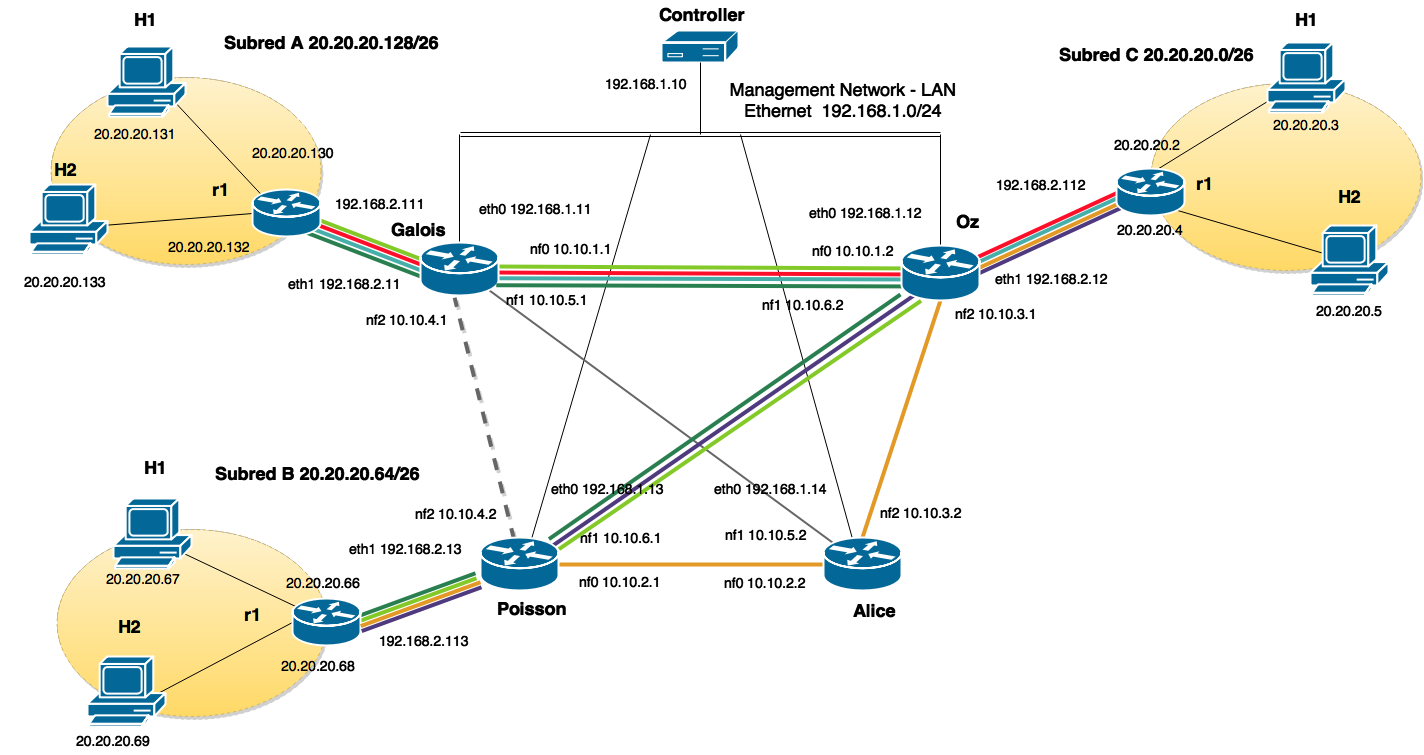
\includegraphics[width=1.0\textwidth]{CU1P1CaminosRecalculo}
\caption[Escenario 1 - Caminos para servicios recalculados]{Escenario 1 - Caminos para servicios recalculados}
\label{fig:CUP1Caminos2}
\end{figure}
 
Notese que los \'unicos caminos que cambian son los asociados a los servicios S3 y S6. Cabe destacar adem\'as que en la nueva opolog\'ia existe m\'as de un camino de m\'inimo costo para S3. Los caminos $<(Galois, nf0), (Oz, nf1)>$ y $<(Galois, nf0), (Oz, nf2), (Alice, nf0)>$ presentan ambos el costo 4.
Por tanto se tienen dos resultados v\'alidos posibles para la salida del algoritmo de ruteo para este servicio.\\

\begin{figure}[ht!] 
\centering    
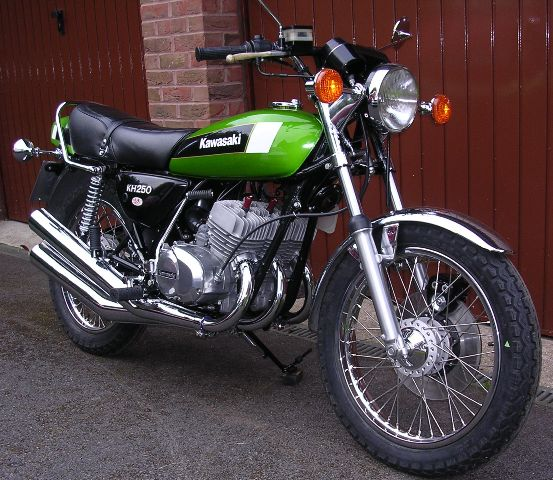
\includegraphics[width=1.0\textwidth]{CU1P1DumpFlows2}
\caption[Cambiar por imagen correcta]{Cambiar por imagen correcta}
\label{fig:CU1P1DumpFlows2}
\end{figure}

\newpage
\subsection{Escenario 2}

Este escenario representa una red privada punto a punto de capa 3. Esta compuesto por dos organizaciones diferentes, cada una de ellas con dos sucursales f\'isicamente separadas.

Se quiere instancia entonces servicios en RAUFlow con el objetivo de brindar conectividad entre cada par de sucursales.
 
\begin{figure}[ht!] 
\centering    
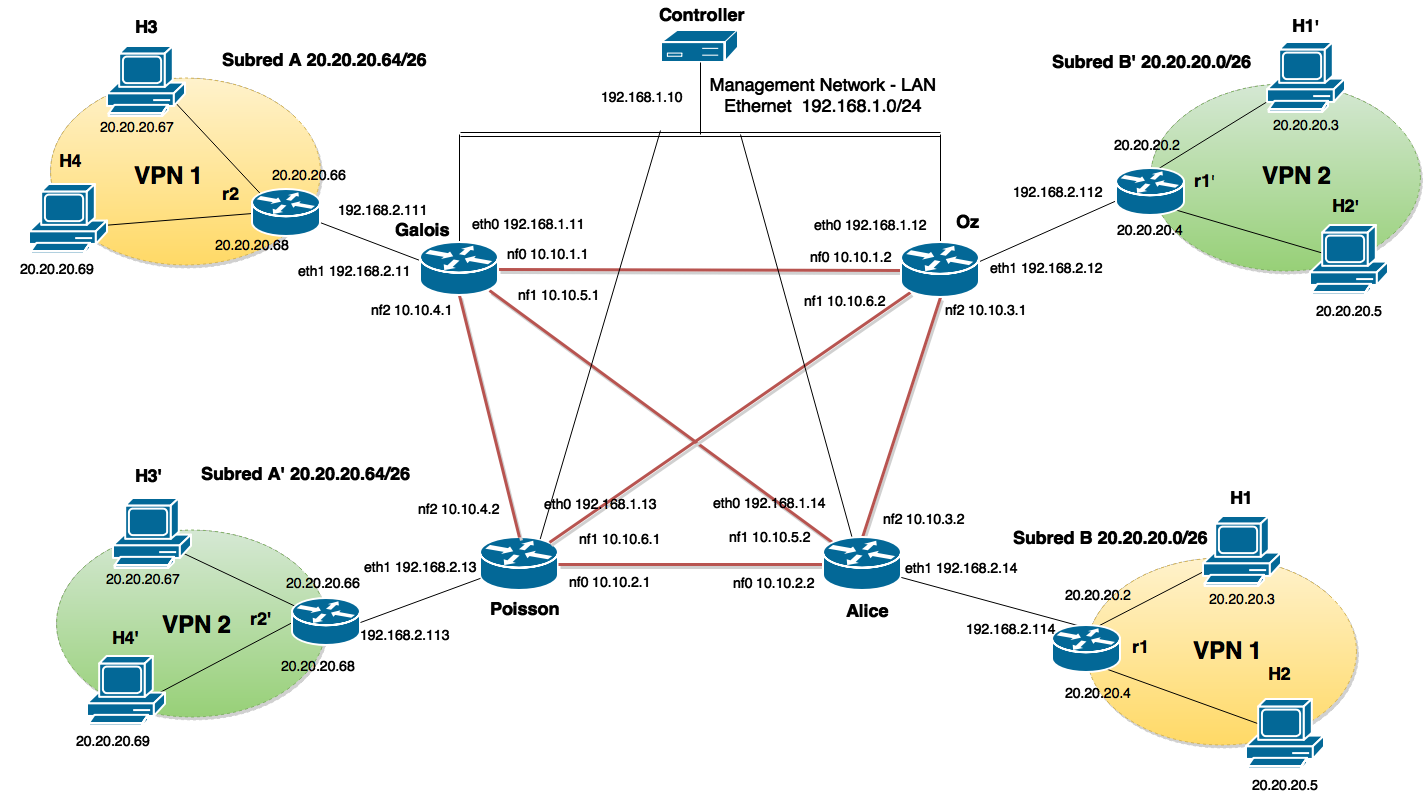
\includegraphics[width=1.0\textwidth]{CU1P2}
\caption[VPN de capa 3 - Escenario 2]{VPN de capa 3 - Escenario 2}
\label{fig:CUP2}
\end{figure}

\section{Pruebas}

\subsection{Asignación de etiquetas}

\subsubsection{Objetivos}
\begin{enumerate}
\item Probar que el algoritmo de distribución de etiquetas funciona correctamente en relación a: (a) asignación de etiquetas identificadoras a nuevos servicios(segundo nivel de etiquetas) y (b) asignación de etiquetas a caminos LSP.
\item Analizar el comportamiento de este algoritmo cuando se prueba con un rango amplio de etiquetas dentro del espacio de etiquetas disponible.
\end{enumerate}

\subsubsection{Descripción de la prueba:}
[Crear muchisimos servicios para utilizar gran parte del arango de etiquetas disponibles. Tomar un muestreo de servicios que utilicen etiquetas que creamos convenientes y analizar el comportamiento del prototipo para el trafico generado en estos servicios en:]

\begin{itemize}
\item Trafico asociado a una VPN es correctamente etiquetado a la entrada del prototipo
\item Trafico asociado a una VPN sale de la red del laboratorio por el nodo de salida y la interfaz de salida prevista, sin etiquetas.
\end{itemize}

\subsubsection{Resultados obtenidos:}

\subsection{Clasificación de tr\'afico}

\subsubsection{Objetivos}
\begin{enumerate}
\item Verificar la clasificación de trafico en base a los matching fields de OpenFlow en los nodos de ingreso
\item Verificar la clasificación de tr\'afico en función a los campos puerto de entrada y etiqueta en los nodos internos(LSRs)
\end{enumerate}

\subsubsection{Descripción de la prueba}
[Hacemos capturas de pantalla en nodos de entrada y en nodos del medio para ver que el trafico se clasifica correctamente. Para esto debemos crear varios servicios]

\subsubsection{Resultados obtenidos}

\subsection{Algoritmo de ruteo dinámico}

\subsubsection{Objetivos:}


\subsubsection{Descripción de la prueba:}


\subsubsection{Resultados obtenidos:}


\subsection{Numeraciones superpuestas}

\textbf{Objetivos}

\textbf{Descripción de la prueba}

\textbf{Resultados obtenidos}